\paragraph{Partie logique} La partie logique possède une partie commune aux 2 applications ainsi qu'une partie individuelle pour l’application banque.

\begin{figure}[ht]
\centering
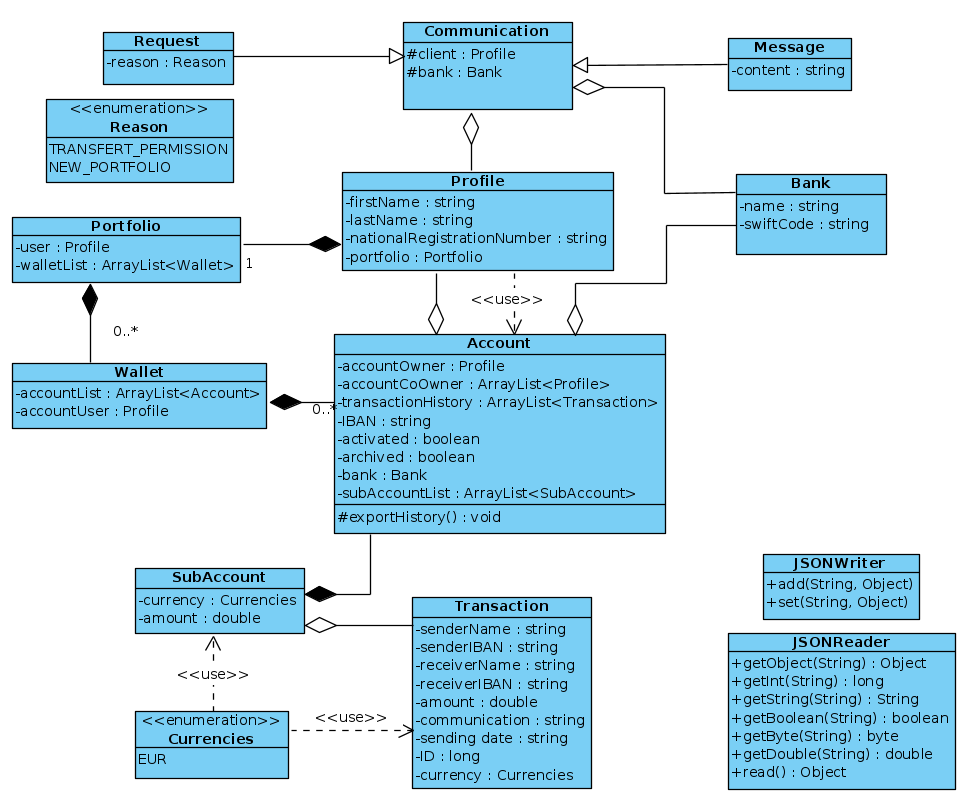
\includegraphics[scale=0.37]{img/ClassCommonPart.png}
\caption{Diagramme de classe de la partie logique commune}
\label{fig1}
\end{figure}

\subparagraph{Partie commune} La partie commune est composée des différents objets qui lient un client à une banque. La classe Profile est la plus utilisée, elle représente un client avec comme attributs le prénom, le nom, le numéro de registre national et son portfolio . Les banques possèdent aussi une classe pour les représenter. Il s’agit de la classe Bank qui a comme attribut un nom et un code Swift. L’utilisation de numéro de registre national et de code swift garantit que le client ou la banque est bien unique. Ensuite, il y a une classe Account qui représente un compte en banque, il possède comme attributs un titulaire, un co-titulaire, un historique de transaction, un IBAN (qui garantit l’unicité du compte), une banque chez laquelle il se trouve, une monnaie, deux booléens qui déterminent si le compte est activé et/ou archivé ainsi qu’une liste de sous compte. Ceux ci font partie de l’extension B mais ont été ajouté dans la partie commue afin de permettre à l’application de base d’intéragir avec la base de donnée qui elle, est commune. Les classes SubAccount et Currencies seront donc expliquées dans l’extension B. La classe Account possède aussi une méthode qui permet d’exporter l’historique de transactions. La classe Transaction possède tous les éléments d’une transaction bancaire, à savoir le nom et l’IBAN de l’envoyeur et du récepteur, le montant de la transaction, une communication, une date d’envoi, un ID et une monnaie. La classe Wallet représente l’ensemble des comptes d’un client chez une même banque. Elle est caractérisée par une liste de compte (objet Account) et d’un utilisateur (objet Profile). La classe Portfolio représente l’ensemble des wallets d’une personne. L’une des dernières classe est la classe Communication. Elle sert à établir des communications entre le client et la banque. Une communication est caractérisée par un client (objet Profile) et une banque (objet Banque). Il s’agit d’une classe mère de 2 classes filles à savoir Request et Message. Request permet au client de créer une requête et à la banque d’y répondre, elle est caractérisée par une énumération de raisons et Message permet à la banque de transmettre un message au client. Enfin, les classes JSONWriter et JSONReader permettent d’écrire et de lire dans des fichiers JSON.


\begin{figure}[ht]
\centering
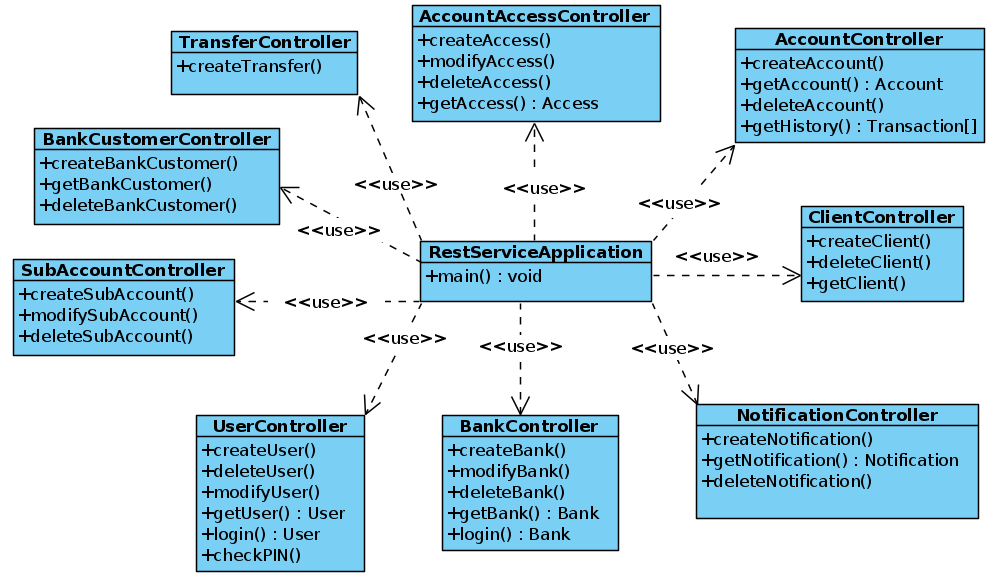
\includegraphics[scale=0.33]{img/APIcommon.png}
\caption{Diagramme de classe de la API commune}
\label{fig2}
\end{figure}

\paragraph{Partie API} La partie API est commune aux 2 applications et permet globalement d’ajouter des données dans la base de données, de les gérer, les supprimer ou les envoyer au client. Tout cela se fait via les classes associées au type de donnée (User, Bank, Account, AccountAccess,Transfer, Client,BankCustomer, SubAccount et Notification) et leur méthode create() qui ajoute, delete() qui supprime, modify() qui modifie et get() qui envoie les données au client.

\newpage

\begin{figure}[ht]
\centering
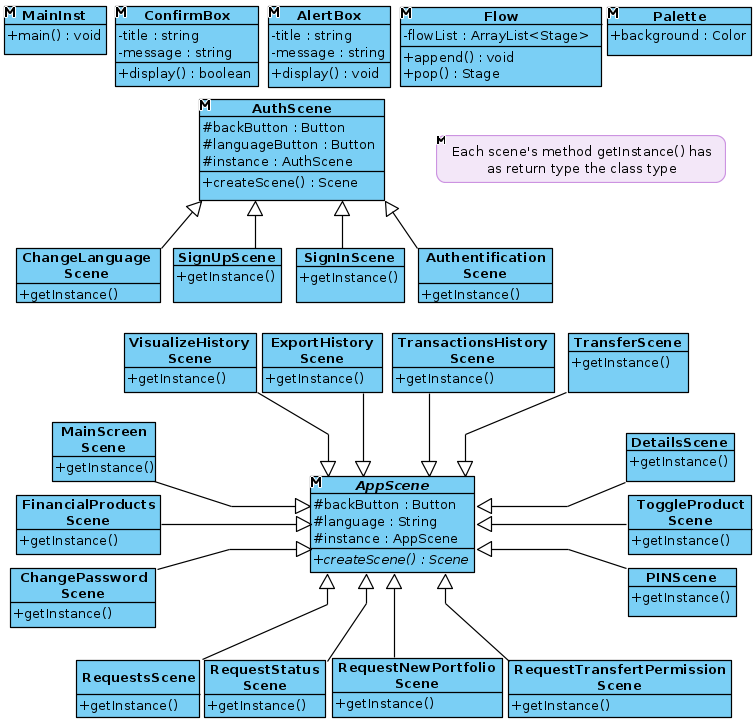
\includegraphics[scale=0.4]{img/GUICLientCommon.png}
\caption{Diagramme de classe de la partie GUI commune}
\label{fig3}
\end{figure}

\paragraph{Partie GUI} La partie GUI est composée de toutes les classes de scenes ainsi que des classes “outil”. Les classes scenes ont toutes la même structure mais il en existe deux sortes. La première sorte est composée des scenes d’authentification (AuthScene) et la deuxième est composée des scenes de l’application une fois connecté (AppScene). La seule différence entre elles est la présence d’un bouton pour changer la langue dans les scenes d’authentification. Les classes abstraites AppScene et AuthScene ont en commun comme caractéristique un bouton de retour ainsi que la langue utilisé dans les fenêtres et comme méthode la méthode createScene qui crée le contenu de la page en fonction de la page sur laquelle on se trouve. Le design patern singleton a été utilisé pour les scenes. En effet, chaque classe Scene possède une méthode statique getInstance() qui permet de garantir qu’il n’existe qu’une instance de l’objet en cours d’utilisation. Pour les classes “outils”, on a ConfirmBox, AlertBox, Flow et Palette. AlertBox et ConfirmBox représentent des fenêtres d’alerte et de confirmation. Elles ont comme attribut un titre et un message et ont comme méthode la méthode display() qui affiche cette fenêtre et renvoie un booléen dans le cas de confirm box. La classe Flow représente une liste de toutes les pages parcourues et sert pour l’utilisation du bouton back, elle a comme attribut une liste d’élément Stage et comme méthode les méthodes append() et pop() qui servent à ajouter des éléments en fin de liste et les retirer en les lisants. La méthode Pallette sert pour avoir un fond d’écran de couleur uni défini par son attribut background. Enfin la classe Main sert à lancer l’application.
